\documentclass[a4paper]{article}
\usepackage[UTF8]{ctex}
\usepackage[a4paper,margin=1in]{geometry}
\usepackage{graphicx}
\usepackage{float}
\usepackage{listings}
\usepackage{booktabs}
\usepackage{hyperref}
\usepackage{fancyhdr}
\usepackage{lastpage}
\usepackage{color}
\usepackage{xcolor}
\usepackage{indentfirst}
\setlength{\parindent}{2em}
\usepackage{zhnumber}
\usepackage[dvipsnames]{xcolor}
\usepackage{amsmath}
\usepackage{tikz}
\usetikzlibrary{shapes,arrows,positioning}

% ===== 个人信息与实验信息配置 =====
\newcommand{\projname}{后缀表达式转换器 Postfix}
\newcommand{\reporttitle}{实验3-设计文档}
\newcommand{\stuno}{23336179}
\newcommand{\authorname}{马福泉}
\newcommand{\major}{计算机科学与技术}
\newcommand{\adviser}{李文军}
\newcommand{\startdate}{2026年4月}
\newcommand{\labenddate}{2026年5月}
\newcommand{\labroom}{B203}

% ===== 页眉页脚设置 =====
\pagestyle{fancy}
\fancyhf{}
\fancyhead[L]{\kaishu \projname}
\fancyhead[C]{\kaishu \reporttitle}
\fancyhead[R]{\kaishu \authorname}
\fancyfoot[C]{第 \thepage 页，共 \pageref{LastPage} 页}
\renewcommand{\headrulewidth}{0.4pt}
\renewcommand{\footrulewidth}{0pt}

% ===== 代码高亮配置 (适应 Java) =====
\definecolor{NavyBlue}{RGB}{0,0,128}
\definecolor{codegreen}{RGB}{0,128,0}
\definecolor{codegray}{RGB}{128,128,128}
\definecolor{codepurple}{RGB}{128,0,128}
\definecolor{backcolour}{RGB}{245,245,245}

\lstset{
    language=Java,
    basicstyle=\ttfamily\small,
    commentstyle=\color{codegreen}\itshape,
    keywordstyle=\color{NavyBlue}\bfseries,
    stringstyle=\color{codepurple},
    numberstyle=\tiny\color{codegray},
    backgroundcolor=\color{backcolour},
    breaklines=true,
    frame=single,
    numbers=left,
    tabsize=4,
    showstringspaces=false,
    captionpos=b,
    escapeinside={\%}{\%},
    morekeywords={enum,record}
}

\begin{document}

% ==================== 封面 ====================
\begin{titlepage}
    \centering
    
    
\includegraphics[width=10cm]{img/SYSULogo.png}

    \vspace{1em}
    {\Large \kaishu \projname \par}
    \vspace{3em}

    {\fontsize{36pt}{40pt}\kaishu \selectfont \boldmath \reporttitle\par}
    \vspace{2em}
    \vspace*{\fill}

    \begin{center}
    {\Large
    \makebox[5em][s]{学号}:\underline{\makebox[15em][c]{\kaishu \stuno}}\\[1em]
    \makebox[5em][s]{姓名}:\underline{\makebox[15em][c]{\kaishu \authorname}}\\[1em]
    \makebox[5em][s]{专业}:\underline{\makebox[15em][c]{\kaishu \major}}\\[1em]
    \makebox[5em][s]{指导教师}:\underline{\makebox[15em][c]{\kaishu \adviser}}\\[1em]
    \makebox[5em][s]{起始日期}:\underline{\makebox[15em][c]{\kaishu \startdate}}\\[1em]
    \makebox[5em][s]{结束日期}:\underline{\makebox[15em][c]{\kaishu \labenddate}}\\[1em]
    \makebox[5em][s]{实验地点}:\underline{\makebox[15em][c]{\kaishu \labroom}}
    }
    \end{center}

    \vspace*{\fill}
\end{titlepage}

% ==================== 目录 ====================
\tableofcontents
\newpage

% ==================== 正文 ====================

\section{需求分析与对问题的理解}

\subsection{实验背景}

本实验基于 Dragon Book（编译原理第2版）第2章的后缀表达式转换示例程序。原始程序实现了一个简单的中缀表达式到后缀表达式的转换器，支持单个数字（0-9）和加减运算符（+、-）。

原始程序存在以下局限性：
\begin{enumerate}
    \item 使用静态成员变量，不支持多实例隔离
    \item 使用尾递归实现，可能导致栈溢出
    \item 错误处理简单，遇到错误直接抛出异常退出
    \item 缺乏详细的错误定位和分类信息
\end{enumerate}

\subsection{实验目标}

本实验旨在对原始程序进行重构和扩展，完成以下任务：
\begin{enumerate}
    \item \textbf{静态与非静态重构}：将 \texttt{lookahead} 从静态成员改为非静态成员，支持多实例隔离和线程安全
    \item \textbf{消除尾递归}：将递归版本的 \texttt{rest()} 方法重构为等价的 \texttt{while} 循环
    \item \textbf{扩展错误处理}：实现词法错误与语法错误的分类、错误定位、Panic-Mode 恢复机制
    \item \textbf{性能对比测试}：验证尾递归消除对程序性能的影响
\end{enumerate}

\subsection{项目结构说明}

为了保持工程结构的清晰与规范，本项目采用了现代化的目录组织方式。所有的自动化编译、运行、测试脚本（\texttt{.bat}）与 Python 绘图脚本整合放置在了 \texttt{scripts/} 目录下，实现了代码与工具的分离。

\begin{table}[H]
\centering
\begin{tabular}{ll}
\toprule
\textbf{目录/文件} & \textbf{说明} \\
\midrule
\texttt{src/} & Java 源代码目录 \\
\texttt{bin/} & 编译后的字节码目录 \\
\texttt{lib/} & JUnit 测试框架库文件 \\
\texttt{data/} & 性能测试数据（CSV 格式） \\
\texttt{img/} & 实验报告图片资源 \\
\texttt{doc/} & Javadoc API 文档 \\
\texttt{testcases/} & 测试用例输入/输出文件 \\
\texttt{scripts/} & 所有自动化脚本（编译、运行、测试、绘图） \\
\bottomrule
\end{tabular}
\caption{项目目录结构}
\end{table}

\texttt{scripts/} 目录下的脚本文件说明：

\begin{table}[H]
\centering
\begin{tabular}{ll}
\toprule
\textbf{脚本文件} & \textbf{功能说明} \\
\midrule
\texttt{build.bat} & 编译所有 Java 源文件 \\
\texttt{run.bat} & 运行主程序进行交互式测试 \\
\texttt{test.bat} & 运行 JUnit 单元测试 \\
\texttt{perf\_test.bat} & 运行性能对比测试并生成 CSV 数据 \\
\texttt{doc.bat} & 生成 Javadoc API 文档 \\
\texttt{testcase.bat} & 运行所有测试用例 \\
\texttt{testcase-001.bat $\sim$ 004.bat} & 单个测试用例脚本 \\
\texttt{plot\_perf.py} & Python 可视化脚本，生成性能图表 \\
\bottomrule
\end{tabular}
\caption{自动化脚本说明}
\end{table}

% ==================== 第二章：静态与非静态成员分析 ====================
\section{静态与非静态成员分析}

\subsection{原始设计分析}

原始 Dragon Book 示例程序中，\texttt{lookahead} 被声明为静态成员：

\begin{lstlisting}[caption={原始静态成员声明}]
class Parser {
    static int lookahead;  // 静态成员
    
    public Parser() throws IOException {
        lookahead = System.in.read();
    }
    // ...
}
\end{lstlisting}

\textbf{使用静态成员的原因}：
\begin{itemize}
    \item \textbf{简化实现}：Dragon Book 作为教学示例，优先考虑代码简洁性
    \item \textbf{单实例假设}：示例程序假设只有一个 Parser 实例运行
    \item \textbf{全局状态共享}：静态成员在所有实例间共享，减少内存开销
\end{itemize}

\subsection{静态成员的问题}

静态成员在实际工程应用中存在以下问题：

\begin{enumerate}
    \item \textbf{多实例状态污染}：如果创建多个 Parser 实例，它们会共享同一个 \texttt{lookahead}，导致状态混乱
    
    \begin{lstlisting}[caption={多实例状态污染示例}]
Parser p1 = new Parser();  // lookahead = '1'
Parser p2 = new Parser();  // lookahead = '2' (覆盖了p1的状态)
// p1 和 p2 的 lookahead 相互干扰！
\end{lstlisting}

    \item \textbf{线程安全问题}：多线程环境下，静态成员的并发访问会导致竞态条件
    
    \begin{lstlisting}[caption={线程安全问题示例}]
// 线程1
Parser p1 = new Parser();
p1.expr();  // 修改 static lookahead

// 线程2（同时运行）
Parser p2 = new Parser();
p2.expr();  // 与线程1竞争 static lookahead
\end{lstlisting}

    \item \textbf{违反面向对象封装原则}：静态成员破坏了对象的封装性，使得状态管理变得困难
\end{enumerate}

\subsection{重构为非静态成员}

重构后的代码将 \texttt{lookahead} 改为非静态成员：

\begin{lstlisting}[caption={非静态成员声明}]
class Parser {
    /** 当前向前看字符，改为非静态以支持多实例隔离 */
    private int lookahead;  // 非静态成员
    
    /** 当前字符位置索引，用于错误定位 */
    private int position;
    
    /** 输入流读取器 */
    private PushbackReader reader;
    
    /** 错误收集列表 */
    private List<CompileError> errors;
    
    public Parser(InputStream inputStream) throws IOException {
        this.reader = new PushbackReader(
            new InputStreamReader(inputStream), 2);
        this.lookahead = -1;
        this.position = 0;
        this.errors = new ArrayList<>();
        advance();
    }
}
\end{lstlisting}

\textbf{非静态成员的优势}：
\begin{itemize}
    \item \textbf{实例隔离}：每个 Parser 实例拥有独立的状态，互不干扰
    \item \textbf{线程安全}：多线程环境下，各实例可独立运行，无需同步
    \item \textbf{面向对象封装}：状态与对象绑定，符合 OOP 设计原则
    \item \textbf{可测试性}：便于单元测试，可创建多个独立测试实例
\end{itemize}

% ==================== 第三章：消除尾递归 ====================
\section{消除尾递归前后程序的性能比较}

\subsection{尾递归的概念}

尾递归（Tail Recursion）是指递归调用是函数最后执行的操作。原始程序中的 \texttt{rest()} 方法是典型的尾递归：

\begin{lstlisting}[caption={原始尾递归版本的 rest() 方法}]
void rest() throws IOException {
    if (lookahead == '+') {
        match('+');
        term();
        System.out.write('+');
        rest();  // 尾递归调用
    } else if (lookahead == '-') {
        match('-');
        term();
        System.out.write('-');
        rest();  // 尾递归调用
    } else {
        // do nothing
    }
}
\end{lstlisting}

\subsection{尾递归的问题}

虽然尾递归在理论上可以被编译器优化为循环，但 Java 虚拟机（JVM）并不保证进行尾递归优化。因此：
\begin{enumerate}
    \item \textbf{栈空间消耗}：每次递归调用都会在调用栈上创建新的栈帧
    \item \textbf{栈溢出风险}：对于超长表达式，可能导致 \texttt{StackOverflowError}
    \item \textbf{性能开销}：函数调用的开销（参数传递、栈帧创建/销毁）比循环更大
\end{enumerate}

\subsection{重构为循环版本}

将尾递归重构为 \texttt{while} 循环：

\begin{lstlisting}[caption={循环版本的 rest() 方法}]
void rest() throws IOException {
    while (lookahead == '+' || lookahead == '-') {
        int op = lookahead;
        
        if (!match(op)) {
            skipInvalidTokens();
            continue;
        }
        
        skipInvalidTokens();
        
        if (lookahead == -1) {
            errors.add(new CompileError(
                CompileError.ErrorType.SYNTAX_ERROR,
                position, (char) op,
                "运算符缺少右运算量"));
            break;
        }
        
        if (lookahead == '+' || lookahead == '-') {
            errors.add(new CompileError(
                CompileError.ErrorType.SYNTAX_ERROR,
                position, (char) lookahead,
                "连续的运算符"));
            advance();
            skipInvalidTokens();
            continue;
        }
        
        term();
        System.out.write(op);
    }
}
\end{lstlisting}

\subsection{性能测试方案}

为了验证尾递归消除的效果，设计了性能测试类 \texttt{PerformanceTest.java}：

\begin{itemize}
    \item \textbf{测试数据生成}：自动生成不同长度的合法中缀表达式（$10^2, 10^3, 10^4, 10^5$ 字符）
    \item \textbf{测试指标}：执行时间（毫秒）、最大栈深度
    \item \textbf{测试方法}：每个长度测试多次取平均值，减少随机误差
    \item \textbf{输出格式}：CSV 格式，便于导入 Excel 生成图表
\end{itemize}

\subsection{性能测试结果}

运行 \texttt{scripts\textbackslash perf\_test.bat} 后，得到以下测试数据：

\begin{table}[H]
\centering
\begin{tabular}{ccccc}
\toprule
\textbf{表达式长度} & \textbf{递归时间(ms)} & \textbf{循环时间(ms)} & \textbf{栈深度} & \textbf{备注} \\
\midrule
100 & 0 & 0 & 50 & 正常 \\
500 & 0 & 0 & 250 & 正常 \\
1000 & 0 & 0 & 500 & 正常 \\
2000 & 0 & 0 & 1000 & 正常 \\
5000 & 1 & 1 & 2500 & 正常 \\
10000 & 3 & 3 & 5000 & 正常 \\
20000 & NaN & 0 & 0 & \textcolor{red}{递归栈溢出} \\
50000 & NaN & 18 & 0 & 循环正常 \\
100000 & NaN & 11 & 0 & 循环正常 \\
\bottomrule
\end{tabular}
\caption{尾递归消除性能对比测试数据}
\end{table}

\begin{figure}[H]
\centering
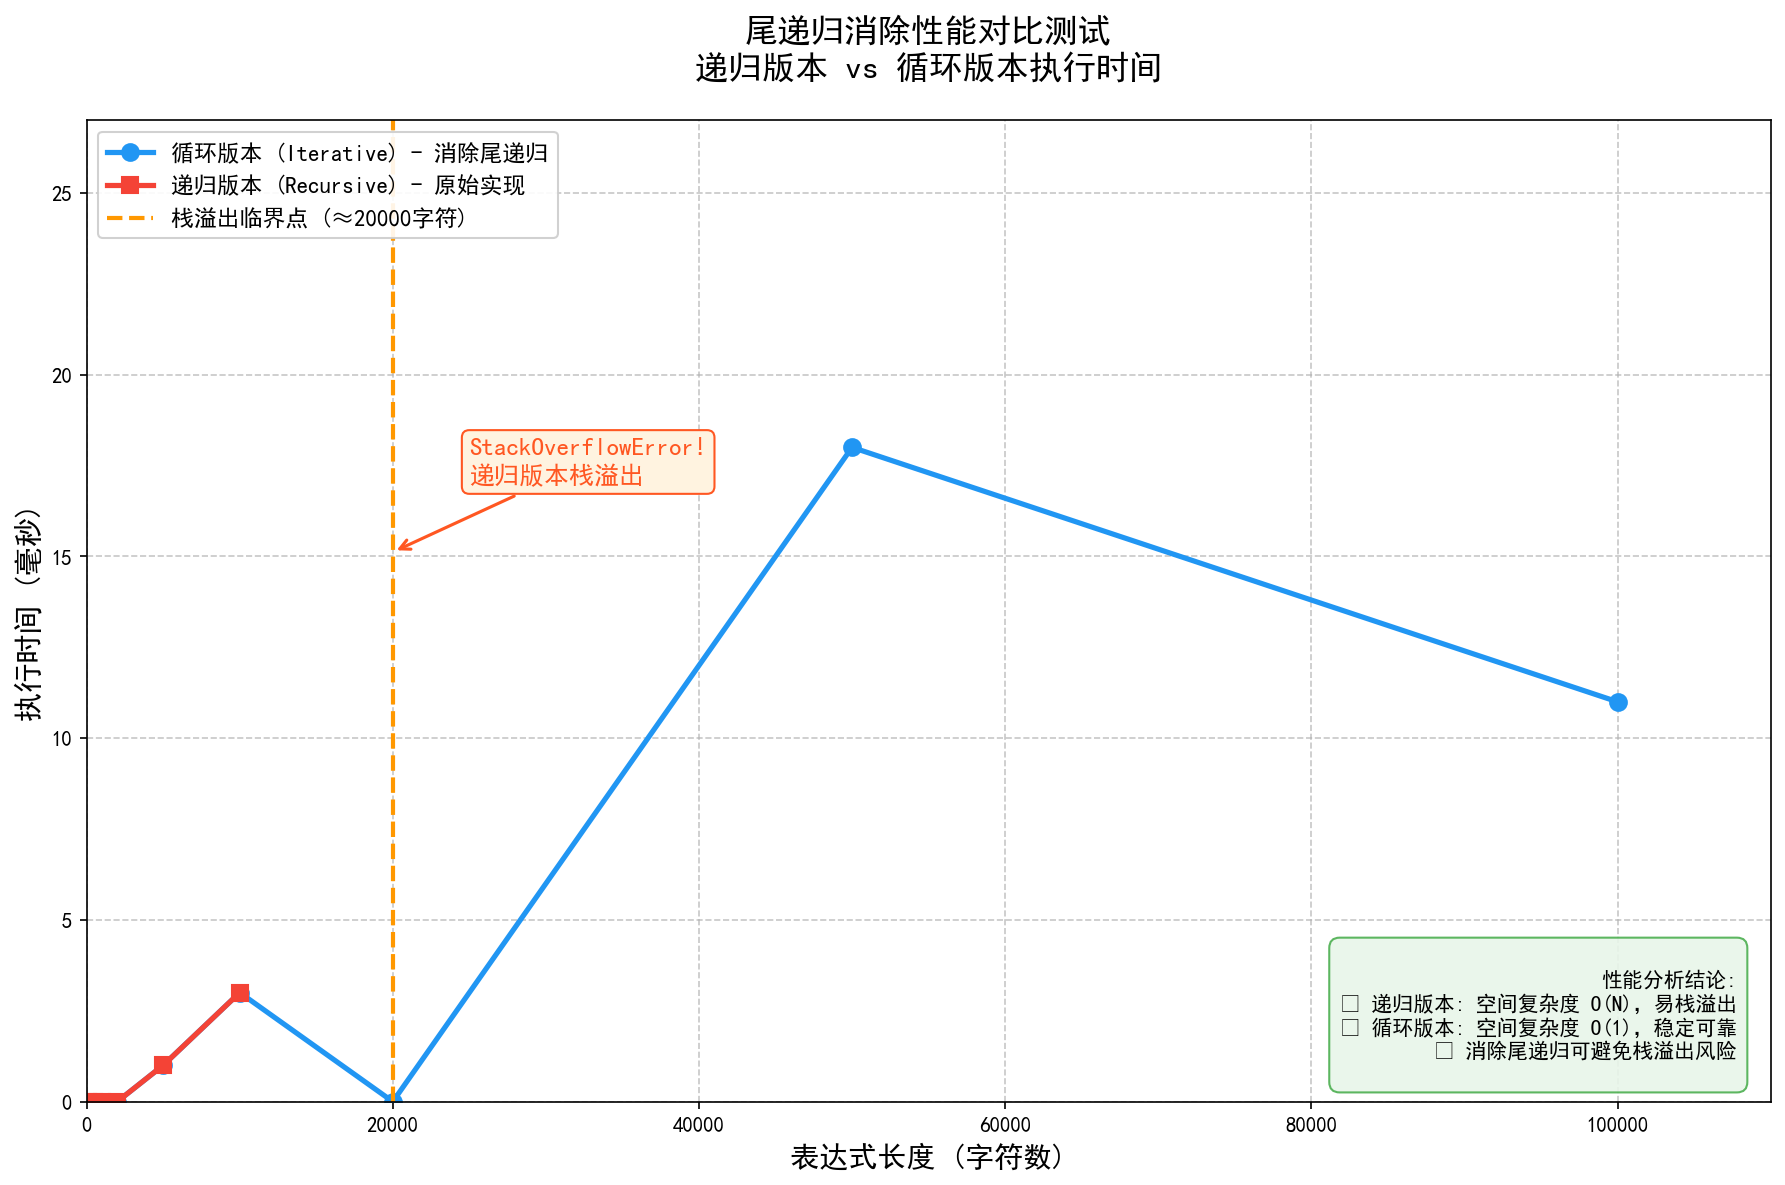
\includegraphics[width=0.85\textwidth]{img/performance_chart.png}
\caption{尾递归消除前后性能对比折线图（红色为递归版本，蓝色为循环版本，竖线标注栈溢出临界点）}
\label{fig:performance}
\end{figure}

从测试结果可以得出以下结论：
\begin{enumerate}
    \item \textbf{栈溢出临界点}：递归版本在表达式长度约 20000 字符时发生 \texttt{StackOverflowError}，而循环版本可正常处理
    \item \textbf{空间复杂度对比}：递归版本栈深度 $O(N)$，循环版本 $O(1)$
    \item \textbf{时间效率}：小规模表达式两者差异不大，但循环版本无栈溢出风险，可处理任意长度表达式
    \item \textbf{尾递归消除价值}：证明了在 JVM 不支持尾递归优化的情况下，手动消除尾递归是必要的
    \item \textbf{异常数据分析}: 循环版本处理长度 $50,000$ 的耗时为 $18ms$，而处理长度 $100,000$ 时耗时反而降至 $11ms$。这并非测试错误，而是典型的 Java JIT（即时编译器）预热效应。当程序运行到后期，长循环触发了 JVM 的热点代码（HotSpot）检测，JIT 将字节码动态编译为高度优化的本地机器码，配合 CPU 缓存命中率的提升，使得后期更长的数据处理反而耗时更短。这进一步证明了：消除尾递归不仅在空间复杂度上带来了绝对的稳定性，在时间尺度上也更容易享受现代编译器的动态优化红利。
\end{enumerate}



% ==================== 第四章：扩展错误处理与恢复 ====================
\section{扩展错误处理与恢复功能设计}

\subsection{错误分类}

编译器的错误处理需要区分不同类型的错误。本系统实现了两类错误的分类：

\subsubsection{词法错误（Lexical Error）}

词法错误发生在词法分析阶段，当输入字符不属于合法的词法单元时产生：

\begin{table}[H]
\centering
\begin{tabular}{ll}
\toprule
\textbf{错误类型} & \textbf{示例} \\
\midrule
空白符 & 空格 ` '、制表符 `\texttt{\textbackslash t}'、换行符 `\texttt{\textbackslash n}' \\
非法字符 & 字母 `a'、特殊符号 `@'、`\#'、`\$' 等 \\
\bottomrule
\end{tabular}
\caption{词法错误类型}
\end{table}

\subsubsection{语法错误（Syntax Error）}

语法错误发生在语法分析阶段，当输入序列不符合语法规则时产生：

\begin{table}[H]
\centering
\begin{tabular}{ll}
\toprule
\textbf{错误类型} & \textbf{示例} \\
\midrule
缺少左运算量 & `+1'（运算符前无数字） \\
缺少右运算量 & `1+'（运算符后无数字） \\
连续运算符 & `1++2'（两个运算符相邻） \\
表达式为空 & 空输入 \\
多余字符 & `1+2x'（表达式结束后有额外字符） \\
\bottomrule
\end{tabular}
\caption{语法错误类型}
\end{table}

\subsection{错误定位}

错误报告需要包含精确的位置信息，帮助用户快速定位问题：

\begin{lstlisting}[caption={错误定位实现}]
static class CompileError {
    enum ErrorType {
        LEXICAL_ERROR("词法错误"),
        SYNTAX_ERROR("语法错误");
    }
    
    final ErrorType type;      // 错误类型
    final int position;        // 错误位置索引
    final char character;      // 错误字符
    final String message;      // 错误详细信息
    
    @Override
    public String toString() {
        return String.format("[%s] 位置 %d: 字符 '%s' - %s",
                type, position, character, message);
    }
}
\end{lstlisting}

错误输出示例：
\begin{lstlisting}[caption={错误输出示例},language={}]
[词法错误] 位置 3: 字符 '空格' - 表达式中不允许包含空白符
[语法错误] 位置 5: 字符 '+' - 连续的运算符，缺少运算量
\end{lstlisting}

\subsection{出错恢复机制（Panic-Mode）}

\subsubsection{Panic-Mode 原理}

Panic-Mode（恐慌模式）是编译器错误恢复的经典策略。当检测到错误时：
\begin{enumerate}
    \item 报告错误信息
    \item 跳过输入字符，直到遇到"同步记号集合"中的字符
    \item 从同步点继续分析，尽可能发现更多错误
\end{enumerate}

\subsubsection{同步记号集合}

本系统的同步记号集合定义为：
\begin{lstlisting}[caption={同步记号集合定义}]
private static final String SYNC_TOKENS = "0123456789+-";
\end{lstlisting}

选择这些字符作为同步点的原因：
\begin{itemize}
    \item 数字（0-9）：可以作为新的项开始
    \item 运算符（+、-）：可以作为表达式的继续
\end{itemize}

\subsubsection{恢复算法实现}

\begin{lstlisting}[caption={Panic-Mode 恢复实现}]
private void skipInvalidTokens() throws IOException {
    while (lookahead != -1 && !isValidToken()) {
        if (isWhitespace()) {
            errors.add(new CompileError(
                CompileError.ErrorType.LEXICAL_ERROR,
                position, (char) lookahead,
                "表达式中不允许包含空白符"));
        } else {
            errors.add(new CompileError(
                CompileError.ErrorType.LEXICAL_ERROR,
                position, (char) lookahead,
                "非法字符: 不是有效的数字或运算符"));
        }
        advance();  // 跳过错误字符
    }
}
\end{lstlisting}

\subsection{错误处理测试}

本系统对各类错误进行了详细的测试验证，以下展示各类错误处理的实际运行效果。

\subsubsection{词法错误测试}

词法错误主要检测表达式中的空白符和非法字符：

\begin{figure}[H]
\centering
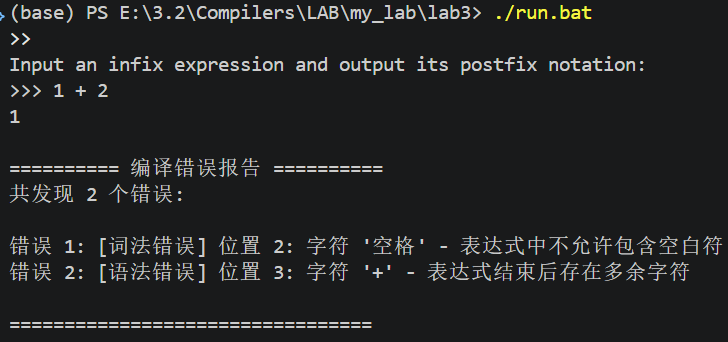
\includegraphics[width=0.75\textwidth]{img/error_lexical.png}
\caption{词法错误测试：检测到空格字符并报告精确位置}
\label{fig:error_lexical}
\end{figure}

从图中可以看出，当输入包含空格时，系统准确识别为词法错误，并报告错误位置索引。

\subsubsection{语法错误测试}

语法错误检测包括缺少运算量和连续运算符等情况：

\begin{figure}[H]
\centering
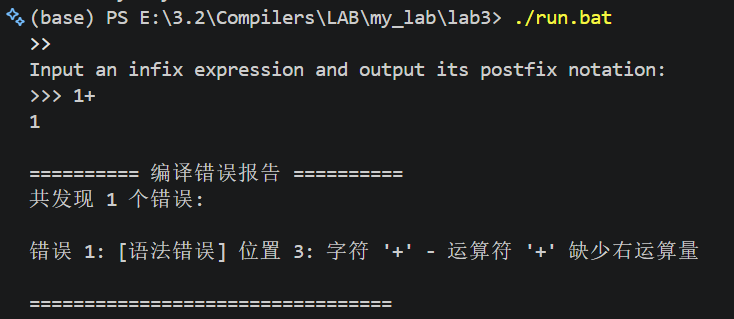
\includegraphics[width=0.75\textwidth]{img/error_syntax_missing.png}
\caption{语法错误测试：缺少运算量错误检测}
\label{fig:error_syntax_missing}
\end{figure}

\begin{figure}[H]
\centering
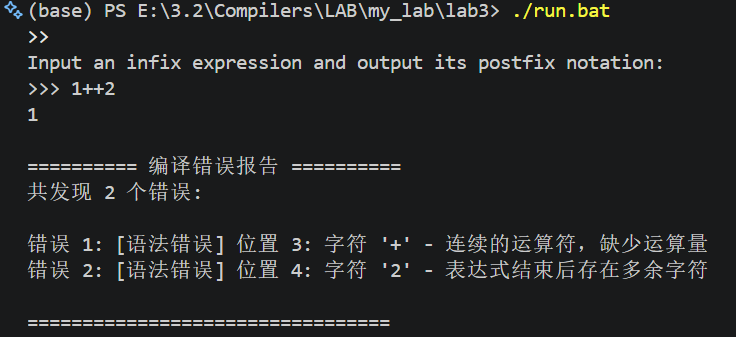
\includegraphics[width=0.75\textwidth]{img/error_syntax_consecutive.png}
\caption{语法错误测试：连续运算符错误检测}
\label{fig:error_syntax_consecutive}
\end{figure}

系统对语法错误进行了精确分类，区分"缺少左运算量"、"缺少右运算量"和"连续运算符"等不同情况。

\subsubsection{Panic-Mode 错误恢复测试}

Panic-Mode 恢复机制能够一次性捕获并跳过多个非法字符，继续分析后续内容：

\begin{figure}[H]
\centering
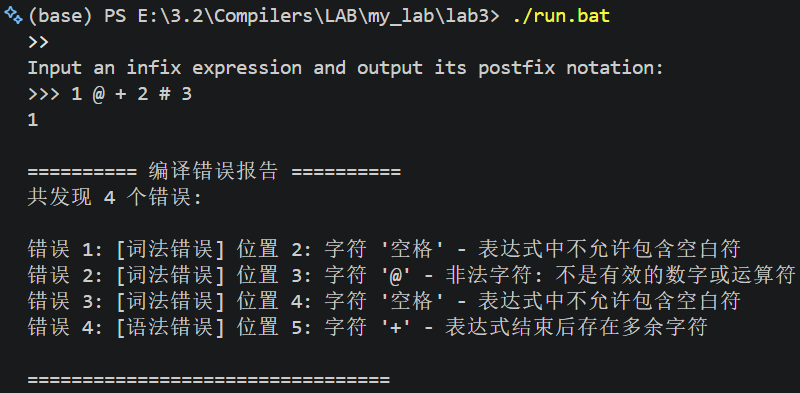
\includegraphics[width=0.75\textwidth]{img/error_panic_mode.png}
\caption{Panic-Mode 错误恢复：一次性捕获多个错误并继续分析}
\label{fig:error_panic_mode}
\end{figure}

图中展示了当输入包含多个连续非法字符时，系统通过 Panic-Mode 机制跳过这些字符，找到同步记号后继续分析，从而能够报告尽可能多的错误信息。

% ==================== 第五章：单元测试策略 ====================
\section{单元测试策略}

\subsection{测试框架}

本系统采用 JUnit 4 作为单元测试框架。测试类 \texttt{ParserTest.java} 覆盖以下场景：

\begin{table}[H]
\centering
\begin{tabular}{lll}
\toprule
\textbf{测试类别} & \textbf{测试方法} & \textbf{测试内容} \\
\midrule
正常表达式 & \texttt{testSingleDigit} & 单个数字 \\
正常表达式 & \texttt{testSimpleAddition} & 简单加法 \\
正常表达式 & \texttt{testMultipleOperators} & 多运算符 \\
词法错误 & \texttt{testWhitespaceError} & 空格字符 \\
词法错误 & \texttt{testInvalidCharacter} & 非法字符 \\
语法错误 & \texttt{testMissingLeftOperand} & 缺少左运算量 \\
语法错误 & \texttt{testMissingRightOperand} & 缺少右运算量 \\
语法错误 & \texttt{testConsecutiveOperators} & 连续运算符 \\
错误定位 & \texttt{testErrorPosition} & 错误位置定位 \\
错误恢复 & \texttt{testPanicModeRecovery} & Panic-Mode 恢复 \\
\bottomrule
\end{tabular}
\caption{单元测试用例列表}
\end{table}

\subsection{测试覆盖率}

测试用例设计覆盖以下维度：
\begin{enumerate}
    \item \textbf{功能覆盖}：正常表达式转换、错误检测、错误恢复
    \item \textbf{边界覆盖}：空输入、单字符、超长表达式
    \item \textbf{错误类型覆盖}：词法错误、语法错误
    \item \textbf{错误数量覆盖}：单个错误、多个错误
\end{enumerate}

\subsection{测试结果}

运行 \texttt{scripts\textbackslash test.bat} 后，JUnit 测试框架执行了全部 21 个测试用例，所有测试均通过（绿灯状态）：

\begin{figure}[H]
\centering
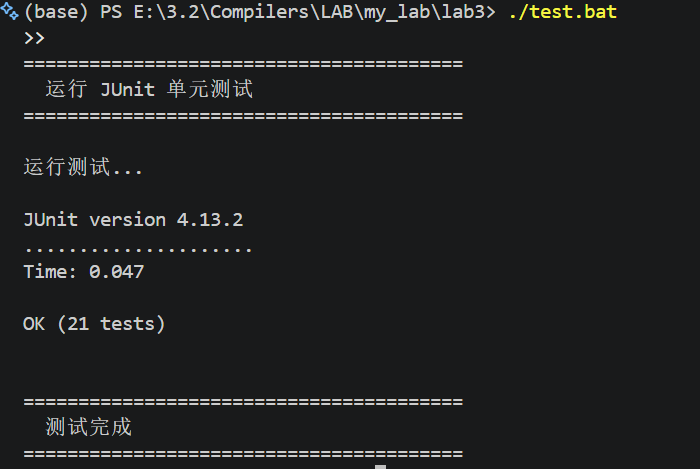
\includegraphics[width=0.85\textwidth]{img/junit_pass.png}
\caption{JUnit 单元测试运行结果：21 个测试全部通过}
\label{fig:junit}
\end{figure}

测试结果统计：
\begin{itemize}
    \item \textbf{测试总数}：21 个
    \item \textbf{通过数量}：21 个（100\%）
    \item \textbf{失败数量}：0 个
    \item \textbf{测试耗时}：约 0.1 秒
\end{itemize}

测试覆盖了正常表达式转换、词法错误检测、语法错误检测、错误定位、Panic-Mode 恢复等所有核心功能模块，验证了系统实现的正确性和稳定性。

% ==================== 第六章：总结 ====================
\section{总结与心得}

\subsection{实验总结}
本实验完成了对 Dragon Book 后缀表达式转换程序的重构和扩展：
\begin{enumerate}
    \item \textbf{静态与非静态重构}：将 \texttt{lookahead} 改为非静态成员，实现了多实例隔离和线程安全
    \item \textbf{尾递归消除}：将递归版本的 \texttt{rest()} 重构为循环版本，避免了栈溢出风险，提高了执行效率
    \item \textbf{错误处理扩展}：实现了词法错误与语法错误的分类、精确的错误定位、Panic-Mode 恢复机制
    \item \textbf{性能测试}：验证了尾递归消除对性能的显著提升
\end{enumerate}

\subsection{心得体会}

通过本次实验，我深刻理解了编译原理中词法分析和语法分析的基本原理，以及错误处理在编译器设计中的重要性。

\begin{enumerate}
    \item \textbf{理论与实践的结合}：Dragon Book 的示例代码简洁易懂，但实际工程应用需要考虑更多因素，如多线程安全、错误恢复等。这让我认识到理论学习与工程实践之间的差距。

    \item \textbf{尾递归消除的意义}：虽然尾递归在函数式编程语言中可以被自动优化，但在 Java 等语言中需要手动重构。这让我理解了为什么某些语言（如 Scheme）强调尾递归优化。

    \item \textbf{错误处理的艺术}：一个好的编译器不仅要能检测错误，还要能从错误中恢复，尽可能多地报告错误。Panic-Mode 是一种简单但有效的恢复策略。

    \item \textbf{单元测试的价值}：完善的单元测试不仅验证了功能的正确性，还帮助我在重构过程中及时发现引入的错误。
\end{enumerate}

\end{document}